\chapter{Transcriptions}
\begin{quotation}
    "Ça ce n'est pas bien, j'ai trois fois sol, même deux fois je m'en prive. Alors bon, exceptionnellement je peux permettre de temps en temps d'avoir deux fois la même note mais c'est vrai que dans les traités tels qu'on les utilise, ceux de par exemple: Marcel Bitsch, Marcel Dupré, les traités du XIXème siècle, on évite, enfin on proscrit même la répétition de la note. Bon et bien ça c'est une règle de bon sens en fait. Ce n'est pas une règle imposée comme ça de manière arbitraire. C'est que le contrepoint doit être une ligne en perpétuel mouvement [\dots]. Attention, chez Fux il le fait, donc c'est intéressant de voir que lui se permet ce genre de choses."
    \textcite[Jean-Louis Fabre's opinion on the repetition of the same note in counterpoint.][1min 11]{ReglesJLFabre}
    \captionof{trans}{French transcription of the video \citetitle{ReglesJLFabre} for rule \ref{rule:codmotions}.}
    \label{appen:JLFabreAvis}
\end{quotation}

Which can be translated as:
\begin{quotation}
    This is not good, I have three times G, even twice I do not use it. So, exceptionally, I can allow from time to time to have the same note twice, but it is true that in the treatises as we use them, those of for example: Marcel Bitsch, Marcel Dupré, the treatises of the XIXth century, we avoid, well we even proscribe the repetition of the note. Well, this is a rule of common sense in fact. It is not a rule imposed arbitrarily. It is that the counterpoint must be a line in perpetual movement [\dots]. Mind you, Fux does this, so it's interesting to see that he allows himself this kind of thing.
    \captionof{trans}{English translation of the above quotation \ref{appen:JLFabreAvis}.}
\end{quotation}
\begin{quotation}
    "[\dots] s'il arrive que cinq noires se suivent par degrés conjoints, soit en montant soit en descendant, la première doit être consonante, la deuxième peut être dissonante, la troisième à nouveau nécessairement consonante, la quatrième pourra être dissonante si la cinquième est une consonance;"
    % \textcite[p.73]{GaPFr}
    \captionof{trans}{Original text from \textcite[p.73]{GaPFr} for rule \ref{rule:fivequarters}.}
    \label{appen:cinqnoires}
\end{quotation}

% \fbox{\centering
%     "[\dots] s'il arrive que cinq noires se suivent par degrés conjoints, soit en montant soit en descendant, la première doit être consonante, la deuxième peut être dissonante, la troisième à nouveau nécessairement consonante, la quatrième pourra être dissonante si la cinquième est une consonance;"
%     \caption{Original text from \textcite[p.73]{GaPFr} on for rule \ref{rule:fivequarters}}
%     }
\begin{quotation}
    "Tertia Contrapuncti Species est quatuor semiminimarum contra unam semibrevem Compositio. Ubi principiò animadvertendum est, quòd, si quinque semiminimas vei ascendendo, vel descendendo \textbf{continuò gradatim} se sequi contingat, prima Consonans esse debeat, secunda dissonans esse possit. Tertia denuo Consonans sit, necesse est. Quarta dissonans esse poterit, \textbf{si} quinta Consonantia fuerit;"
    \captionof{trans}{Original text from \textcite[p.63-64]{IMSLPlatin} for rule \ref{rule:fivequarters}.}
    \label{appen:fuxquinque}
\end{quotation}

\chapter{Additional Material}
% \begin{table}[h]
%     \begin{adjustbox}{angle=90}
%       \begin{tabular}{|c|||c|c|c|c|c|c|c|c|c|c|c|c|}
%       \hline
%       Range & $C$ & $C\sharp$ / $D\flat$ & $D$ & $D\sharp$ / $E\flat$ & $E$ & $F$ & $F\sharp$ / $G\flat$ & $G$ & $G\sharp$ / $A\flat$ & $A$ & $A\sharp$ / $B\flat$ & $B$ \\ \hline \hline
%       -1 & 0 & 1 & 2 & 3 & 4 & 5 & 6 & 7 & 8 & 9 & 10 & 11 \\ \hline
%       0 & 12 & 13 & 14 & 15 & 16 & 17 & 18 & 19 & 20 & \textbf{21} & 22 & 23 \\ \hline
%       1 & 24 & 25 & 26 & 27 & 28 & 29 & 30 & 31 & 32 & 33 & 34 & 35 \\ \hline
%       2 & 36 & 37 & 38 & 39 & 40 & 41 & 42 & 43 & 44 & 45 & 46 & 47 \\ \hline
%       3 & 48 & 49 & 50 & 51 & 52 & 53 & 54 & 55 & 56 & 57 & 58 & 59 \\ \hline
%       4 & 60 & 61 & 62 & 63 & 64 & 65 & 66 & 67 & 68 & 69 & 70 & 71 \\ \hline
%       5 & 72 & 73 & 74 & 75 & 76 & 77 & 78 & 79 & 80 & 81 & 82 & 83 \\ \hline
%       6 & 84 & 85 & 86 & 87 & 88 & 89 & 90 & 91 & 92 & 93 & 94 & 95 \\ \hline
%       7 & 96 & 97 & 98 & 99 & 100 & 101 & 102 & 103 & 104 & 105 & 106 & 107 \\ \hline
%       8 & \textbf{108} & 109 & 110 & 111 & 112 & 113 & 114 & 115 & 116 & 117 & 118 & 119 \\ \hline
%       9 & 120 & 121 & 122 & 123 & 124 & 125 & 126 & 127 & - & - & - & - \\ \hline
%       \end{tabular}
%     \end{adjustbox}
%     \caption{MIDI note values.}
%     \label{tab:midivalues}
% \end{table}
\begin{table}[h]
    % \resizebox{\textwidth}{!}{%
    \setlength\tabcolsep{9pt}
    \begin{tabular*}{\linewidth}{@{\extracolsep{\fill}} |c||c|c|c|c|c|c|c|c|c|c|c|}
        % \begin{tabular}{|c|||c|c|c|c|c|c|c|c|c|c|c|}
            \hline
            Range & -1 & 0 & 1 & 2 & 3 & 4 & 5 & 6 & 7 & 8 & 9\\ \hline \hline
            $C$ & 0 & 12 & 24 & 36 & 48 & 60 & 72 & 84 & 96 & 108 & 120 \\ \hline
            $C\sharp$ / $D\flat$ & 1 & 13 & 25 & 37 & 49 & 61 & 73 & 85 & 97 & 109 & 121 \\ \hline
            $D$ & 2 & 14 & 26 & 38 & 50 & 62 & 74 & 86 & 98 & 110 & 122 \\ \hline
            $D\sharp$ / $E\flat$ & 3 & 15 & 27 & 39 & 51 & 63 & 75 & 87 & 99 & 111 & 123 \\ \hline
            $E$ & 4 & 16 & 28 & 40 & 52 & 64 & 76 & 88 & 100 & 112 & 124 \\ \hline
            $F$ & 5 & 17 & 29 & 41 & 53 & 65 & 77 & 89 & 101 & 113 & 125 \\ \hline
            $F\sharp$ / $G\flat$ & 6 & 18 & 30 & 42 & 54 & 66 & 78 & 90 & 102 & 114 & 126 \\ \hline
            $G$ & 7 & 19 & 31 & 43 & 55 & 67 & 79 & 91 & 103 & 115 & 127 \\ \hline
            $G\sharp$ / $A\flat$ & 8 & 20 & 32 & 44 & 56 & 68 & 80 & 92 & 104 & 116 & - \\ \hline
            $A$ & 9 & 21 & 33 & 45 & 57 & 69 & 81 & 93 & 105 & 117 & - \\ \hline
            $A\sharp$ / $B\flat$ & 10 & 22 & 34 & 46 & 58 & 70 & 82 & 94 & 106 & 118 & - \\ \hline
            $B$ & 11 & 23 & 35 & 47 & 59 & 71 & 83 & 95 & 107 & 119 & - \\ \hline
        % \end{tabular}
    % }
    \end{tabular*}
    \caption{MIDI note values.}
    \label{tab:midivalues}
\end{table}

\begin{figure}[h]
    \centering
    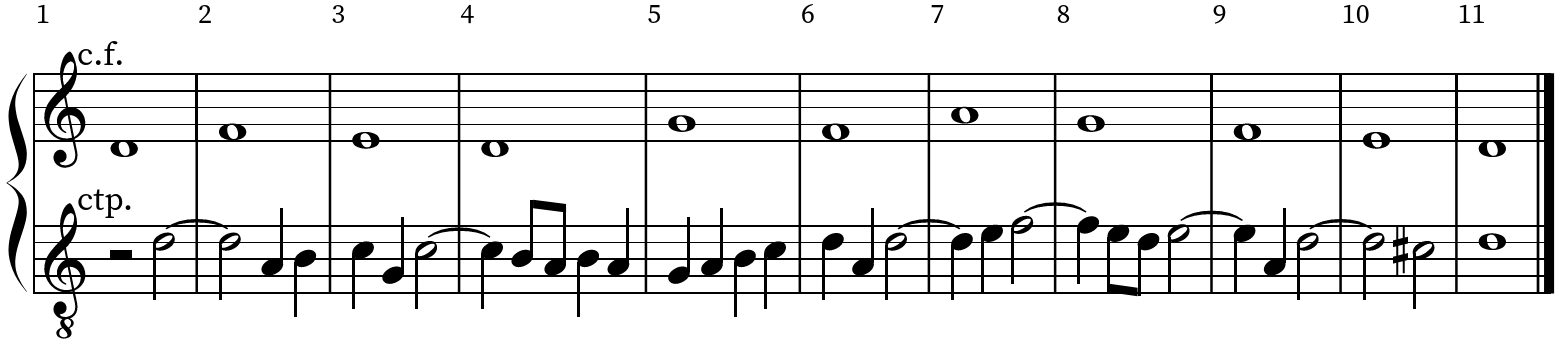
\includegraphics[height=\fhs]{Images/fux_5spB.png}
    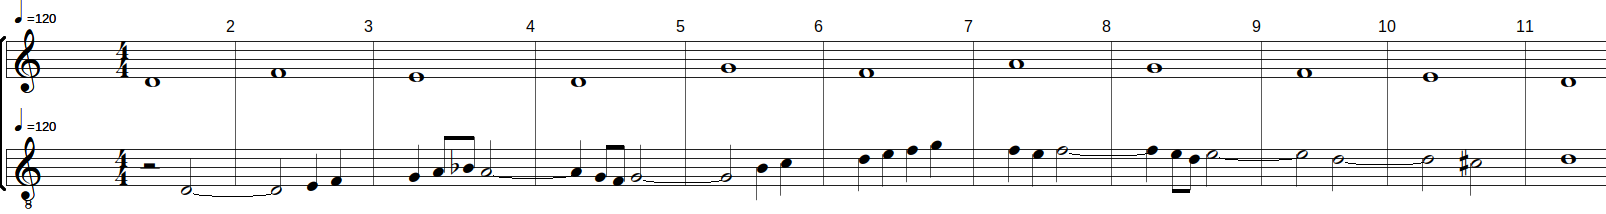
\includegraphics[width=\textwidth, height=1in]{Images/solver_5spB.png}
    \caption{\species{5} upper ctp. of Fux (above) vs. upper ctp. of the solver [2.690 s] (below).}
    \label{fig:eval_5spB}
\end{figure}

\begin{figure}[h]
    \centering
    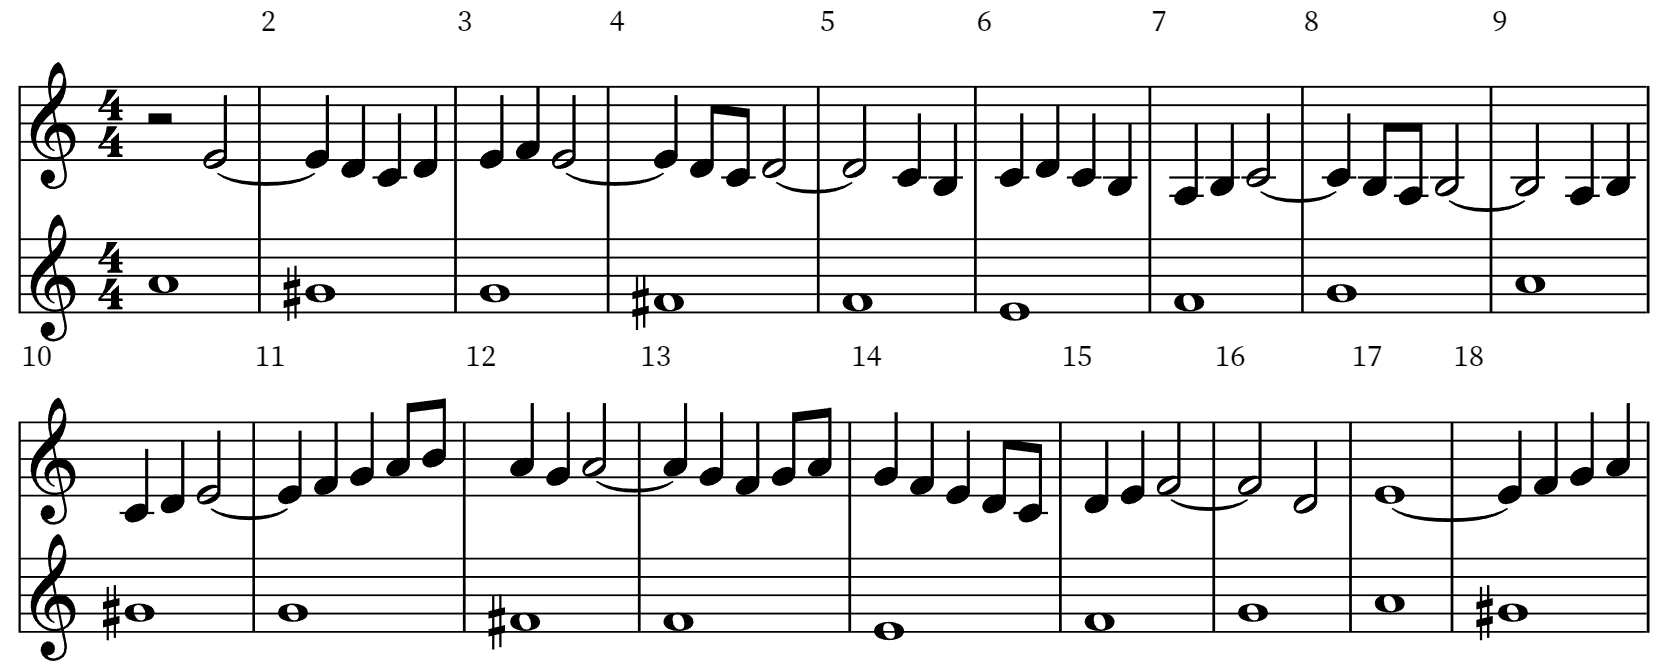
\includegraphics[width=\textwidth]{Images/exp1.png}
    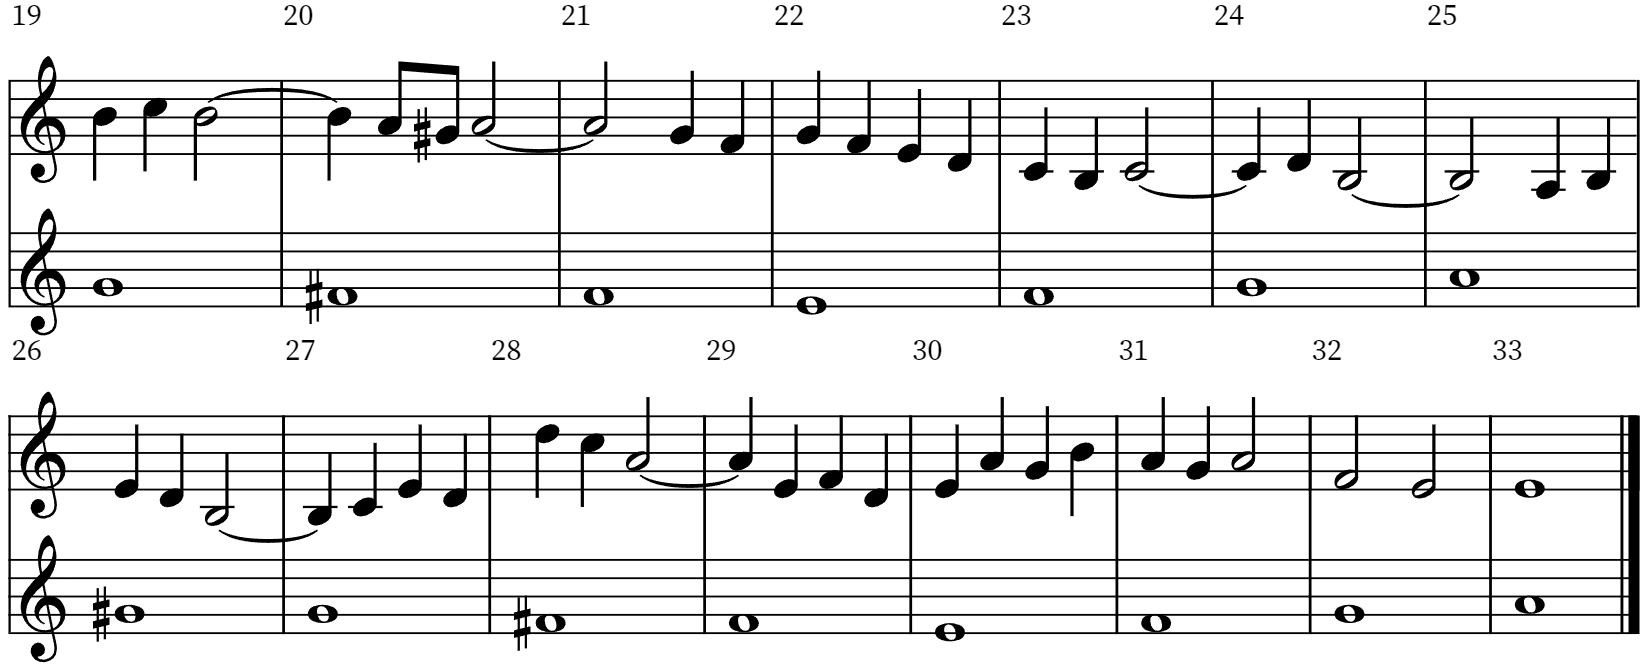
\includegraphics[width=0.99\textwidth]{Images/exp2.png}
    \caption{Solver-generated \species{5} "ctp." with a chromatic "\textit{cantus firmus}".}
    \label{fig:exp_scores}
\end{figure}

\chapter{User Guide}
This user guide provides a overview of FuxCP, covering its installation process, usage within OpenMusic, and a description of the costs displayed in the interface. While FuxCP is designed to be compatible with all platforms, it relies on GiL, which currently works only on MacOS and Linux. Unfortunately, GiL does not support Windows due to compatibility issues between the 32-bit Lisp license used by OpenMusic and the 64-bit Gecode Windows version. Although it is technically possible to obtain a 32-bit version of Gecode for Windows, it is not recommended. 

\section{Installing FuxCP}
\subsection{Prerequisites}
To use FuxCP, it is necessary to download and install the following tools:
\begin{itemize}
    \item Gecode on \url{https://www.gecode.org/download.html}
    \item OpenMusic on \url{https://openmusic-project.github.io/openmusic/}
\end{itemize}

And download the following libraries:
\begin{itemize}
    \item GiL on \url{https://github.com/sprockeelsd/GiLv2.0}
    \item FuxCP : \url{https://github.com/sprockeelsd/Melodizer}
\end{itemize}
On the last github, other tools such as Melodizer and Melodizer2.0 are available. In the context of this user guide, only the FuxCP folder will be necessary.

\subsection{Loading FuxCP in OpenMusic}
To use the previous libraries, OpenMusic must be launched. Upon opening any workspace, locate the toolbar at the top of the interface. Click on the "Windows" button, highlighted in figure \ref{fig:library}, and select "Library" from the dropdown menu. This action will unveil a new window. In the toolbar of this window, choose "File" and then "Add remote library." Navigate through your file system to find the path where the previously downloaded FuxCP and Gil libraries are stored. Once located, the libraries should appear under the "libraries" folder in the "Library" window, as depicted in figure \ref{fig:load}. Right-click on "fuxcp" and select "Load Library". If no errors occur, the setup is complete.

However, if an error arises, it may be a linking issue with the Gecode library. For MacOS users, a script can be used from the \texttt{c++} folder of the gil library. Edit the path to Gecode inside the script to match your system's configuration. Linux users should add the Gecode library to the \texttt{LD\_LIBRARY\_PATH} variable. Go to the \texttt{/etc/ld.so.conf.d} folder and create a new \texttt{.conf} file if one does not already exist. In this file, paste the full path to the Gecode library, save it, and run \texttt{sudo ldconfig} to update the system with the new library. Don't forget to restart OpenMusic and don't stop believing. Following these steps should ensure the proper utilization of FuxCP.

\begin{figure}[h]
    \centering
    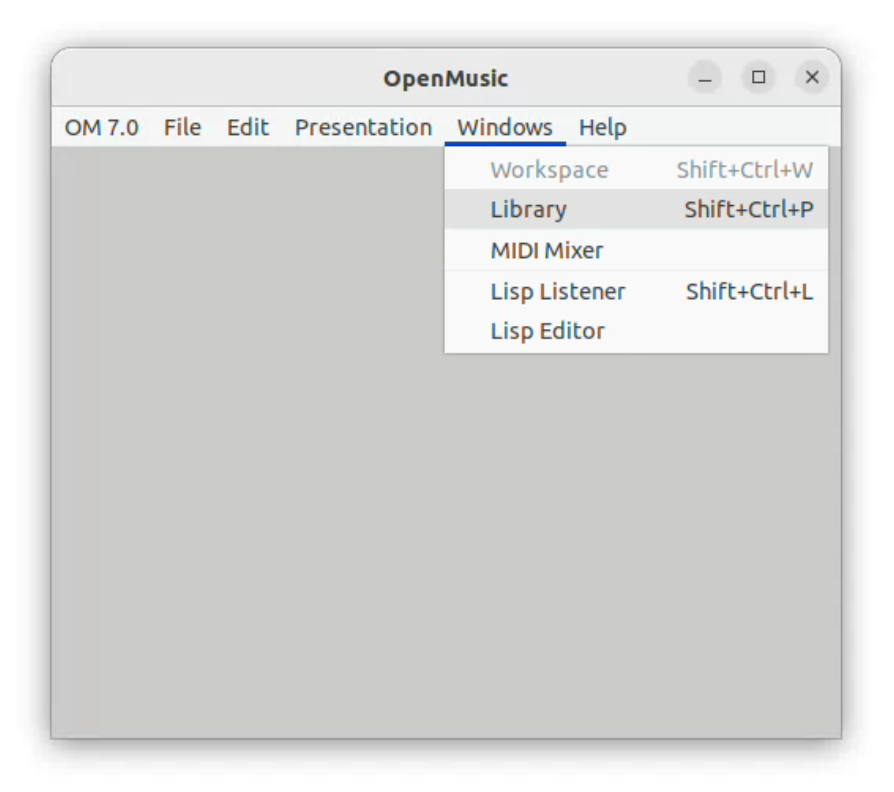
\includegraphics[height=2.6in]{Images/openmusic_library.png}
    \caption{Opening the "Library" window in OpenMusic.}
    \label{fig:library}
\end{figure}
\begin{figure}[h]
    \centering
    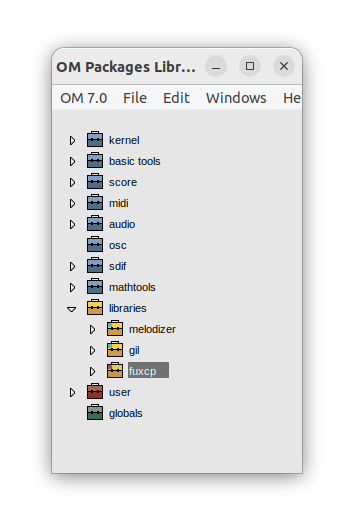
\includegraphics[height=2.6in]{Images/openmusic_load.png}
    \caption{Loading the "fuxcp" library in OpenMusic.}
    \label{fig:load}
\end{figure}

\section{Using FuxCP in OpenMusic}
It is straightforward to use FuxCP in OpenMusic. There is a single block comprising the entire graphical interface of the tool. This block or class is called \texttt{cp-params}. To load it, it is possible to type \texttt{fuxcp::cp-params} in a new patch entry; or load the block of the class by loading "cp-params" from the drop-down menu by right-clicking in the patch ($Classes\to Libraries\to FuxCP\to Solver\to CP-PARAMS$).

Once this block has appeared, all you have to do is bind an OM voice object, representing the \cfcomma to the second argument of \texttt{cp-params} as shown in figure \ref{fig:om_ext_interface_mod}. Don't forget to block the input voice object and evaluate \texttt{cp-params} so it can detect the new input. Now \texttt{cp-params} can be blocked too. From now on, you could directly use the interface and generate counterpoints using the tool. If you want to retrieve the voice object containing the counterpoint generated by the tool, just bind the third argument on the output side to a voice object. Once bound, it is then possible to evaluate the voice object so that it updates.

\begin{figure}[h]
    \centering
    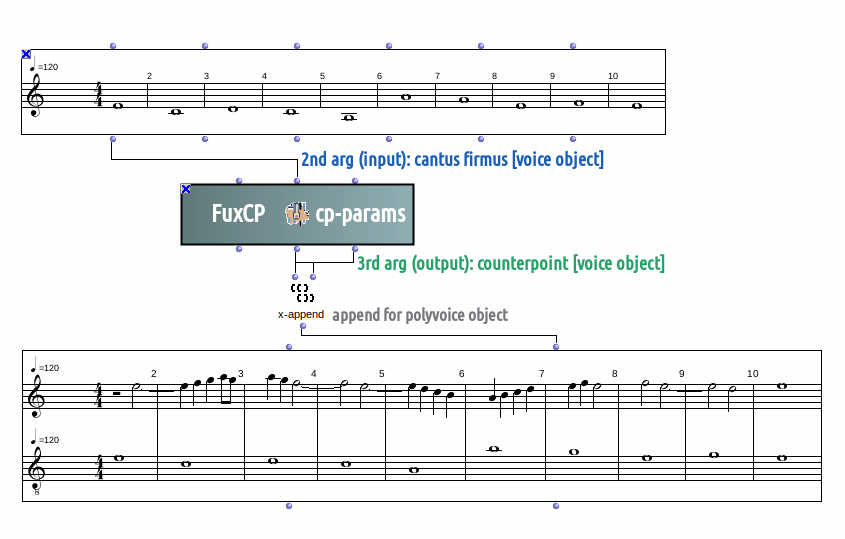
\includegraphics[width=5.2in]{Images/om_ext_interface_mod.png}
    \caption{View of a patch using \texttt{fuxcp::cp-params} in OpenMusic.}
    \label{fig:om_ext_interface_mod}
\end{figure}

But how to use the interface? Just double-click on the block to make it appear. The interface is sorted from left to right, so that the preferences are separated into three different categories: "Preferences for Melodic Intervals of\dots", "General Preferences", "Species Specific Preferences", "Solver Configuration", and in the lower right corner, "Solver Launcher" (see figure \ref{fig:om_int_interface}). Once the preferences have been chosen, the default ones representing the style of Fux, you must save the parameters ("Save Config") in order to then be able to launch the search for a solution ("Next Solution"). This search can take a fraction of a second just as it can take tens of minutes, or even hours if the parameters chosen make the search difficult. If a search takes too long, it is always possible to stop it by clicking on "Stop". You can then either change the preferences in a way (often at the level of the costs of the melodic intervals), or increase the "Irreverence" to obtain potentially less "good" but faster solutions. The description of the parameters is available in the next section.

\begin{figure}[h]
    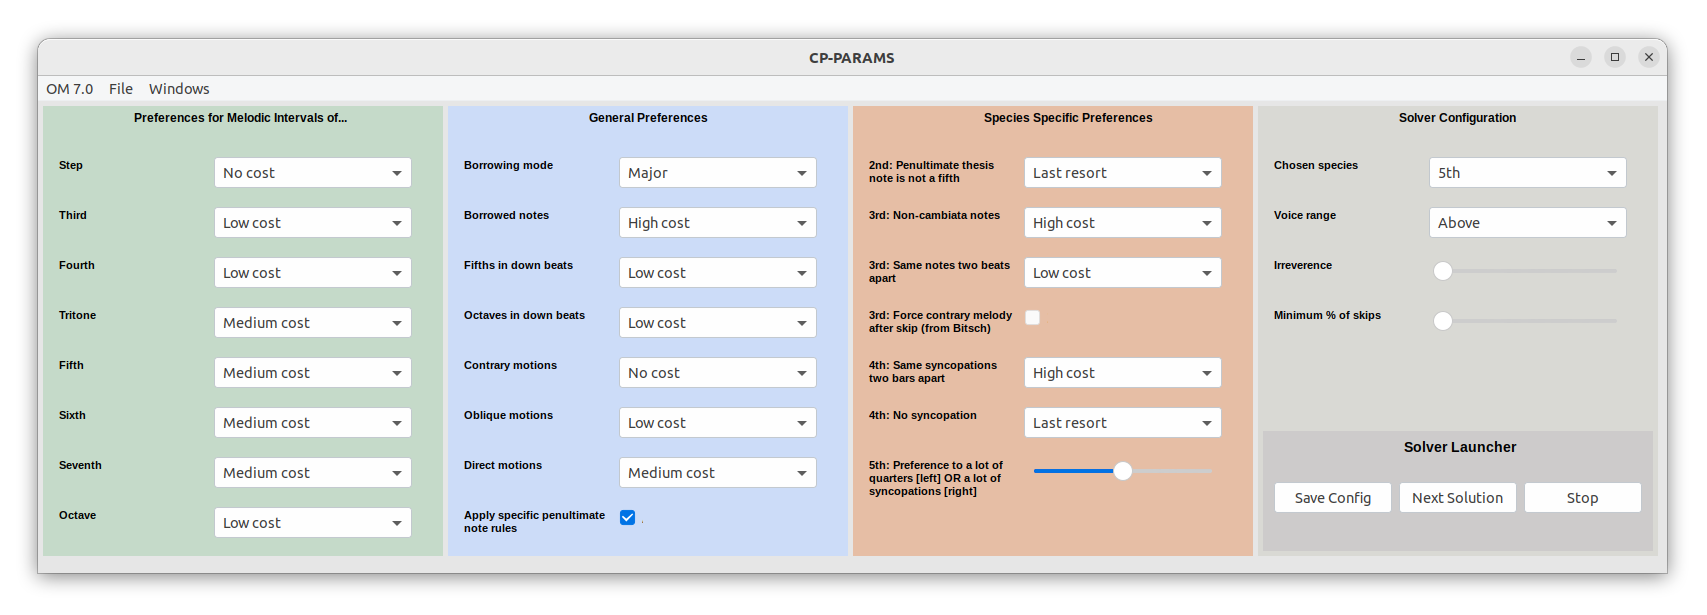
\includegraphics[width=1.4\textwidth, center]{Images/om_int_interface.png}
    \caption{User interface of the \texttt{fuxcp::cp-params} class in OpenMusic.}
    \label{fig:om_int_interface}
\end{figure}

\section{Interface Parameters Description}
Table \ref{tab:cp-params} describes all the parameters available in the interface. A low cost represents a high preference while a high cost represents a low preference.

\begin{table}[!h]
    \footnotesize
    \begin{adjustbox}{center}
        \begin{tabular}{|m{0.22\textwidth}|m{0.82\textwidth}|m{0.15\textwidth}<{\centering}|}
        \hline
        \multicolumn{1}{|c|}{\textbf{Name}} &
          \multicolumn{1}{c|}{\textbf{Description}} &
          \textbf{Default value} \\ \hline
        \cellcolor[HTML]{BCE08D}Step &
          Preference for melodic intervals of one step or less. &
          No cost \\ \hline
        \cellcolor[HTML]{BCE08D}Third &
          Preference for melodic third skips. &
          Low cost \\ \hline
        \cellcolor[HTML]{BCE08D}Fourth &
          Preference for melodic fourth leaps. &
          Low cost \\ \hline
        \cellcolor[HTML]{BCE08D}Tritone &
          Preference for melodic tritone leaps. &
          Forbidden \\ \hline
        \cellcolor[HTML]{BCE08D}Fifth &
          Preference for melodic fifth leaps. &
          Medium cost \\ \hline
        \cellcolor[HTML]{BCE08D}Sixth &
          Preference for melodic sixth leaps. &
          Medium cost \\ \hline
        \cellcolor[HTML]{BCE08D}Seventh &
          Preference for melodic seventh leaps. &
          Medium cost \\ \hline
        \cellcolor[HTML]{BCE08D}Octave &
          Preference for melodic octave leaps. &
          Low cost \\ \hline
        \hline
        \cellcolor[HTML]{C8D6FF}Borrowing mode &
          Type of scale from which notes can be borrowed to generate counterpoint. The first note of the \cf determines the tonic of this scale. Applies everywhere except the penultimate bar. &
          Major \\ \hline
        \cellcolor[HTML]{C8D6FF}Borrowed notes &
          Preference for borrowed notes outside the diatonic scale. These notes are defined by the "Borrowing mode" parameter. &
          High cost \\ \hline
        \cellcolor[HTML]{C8D6FF}Fifths in down beats &
          Preference to have harmonic fifths on the first beat of a bar. &
          Low cost \\ \hline
        \cellcolor[HTML]{C8D6FF}Octaves in down beats &
          Preference to have harmonic octaves on the first beat of a bar. &
          Low cost \\ \hline
        \cellcolor[HTML]{C8D6FF}Contrary motions &
          Preference to have, between two bars, one voice rising while the other is falling. &
          No cost \\ \hline
        \cellcolor[HTML]{C8D6FF}Oblique motions &
          Preference to have, between two bars, one static voice while the other is moving. &
          Low cost \\ \hline
        \cellcolor[HTML]{C8D6FF}Direct motions &
          Preference to have, between two bars, the two voices going in the same direction. &
          Medium cost \\ \hline
        \cellcolor[HTML]{C8D6FF}Apply specific penultimate note rules &
          Force all rules on the notes of the penultimate measure. This mainly refers to the penultimate note that must harmonically be either a major sixth or a minor third depending on whether the counterpoint is above or below. &
          Checked \\ \hline
        \hline
        \cellcolor[HTML]{FFCE93}2nd: Penultimate thesis note is not a fifth &
          Preference for the first note of the penultimate bar to be something other than a harmonic fifth &
          Last resort \\ \hline
        \cellcolor[HTML]{FFCE93}3rd: Non-cambiata notes &
          Preference for the second quarter note of a bar to be a consonance already surrounded by two consonances. &
          High cost \\ \hline
        \cellcolor[HTML]{FFCE93}3rd: Same notes two beats apart &
          Preference to have the same quarter notes two beats apart. A high cost allows to avoid a certain monotony. &
          Low cost \\ \hline
        \cellcolor[HTML]{FFCE93}3rd: Force joint contrary melody after skip &
          Force that a melodic skip or leap is followed by a melodic step in the opposite direction. &
          Unchecked \\ \hline
        \cellcolor[HTML]{FFCE93}4th: Same syncopations two bars apart &
          Preference to have the same half notes two bars apart. A high cost allows to avoid a certain monotony. &
          High cost \\ \hline
        \cellcolor[HTML]{FFCE93}4th: No syncopation &
          Preference to have distinct half notes instead of syncopations. &
          Last resort \\ \hline
        \cellcolor[HTML]{FFCE93}5th: Preferences to a lot of quarters or a lot of syncopations &
          Determines the minimum percentage of quarter notes (to the left) and syncopations (to the right) in the fifth species. Pushing the slider all the way to one side is not recommended. &
          <center> \\ \hline
        \hline
        \cellcolor[HTML]{EFEFEF}Chosen species &
          Determines the type of counterpoint that the tool will generate. From whole notes to syncopations, passing through quarter notes. The fifth species uses the rules and preferences of the previous species. &
          5th \\ \hline
        \cellcolor[HTML]{EFEFEF}Voice range &
          Determines around which pitch the counterpoint will be generated depending on the pitch of the first note of the \cfdot &
          Above \\ \hline
        \cellcolor[HTML]{EFEFEF}Irreverence &
          Artificially increases the minimum cost of the solution to obtain counterpoints that are less respectful of the established preferences. Can also be used to get solutions faster. &
          0 \\ \hline
        \cellcolor[HTML]{EFEFEF}Minimum \% of skips &
          Determines, depending on the counterpoint size, the percentage of melodic intervals larger than one step. &
          0\% \\ \hline
        \cellcolor[HTML]{D1D1D1}Save Config &
          Saves all established preferences and allows you to start a new search for this configuration later. &
          - \\ \hline
        \cellcolor[HTML]{D1D1D1}Next Solution &
          Starts or continues searching for the previously saved configuration. Displays a new window with the solution when it is found. Displays an error message if no other solution can be found. &
          - \\ \hline
        \cellcolor[HTML]{D1D1D1}Stop &
          Pause the search. It may take up to 5 seconds. &
          - \\ \hline
        \end{tabular}
    \end{adjustbox}
    \caption{Description of the parameters of \texttt{fuxcp::cp-params}.}
    \label{tab:cp-params}
\end{table}

\chapter{Software Architecture}\label{ch:software_arch}
This appendix summarizes the architecture of the software. First, from the point of view of the role of FuxCP as a tool and second, from the point of view of the organization of the code in FuxCP.

As shown in figure \ref{fig:macro_arch}, FuxCP is an OpenMusic library that uses GiL to communicate constraints with Gecode. The solver itself therefore runs well in Gecode directly. At the level of the distribution of the files (see figure \ref{fig:micro_arch}), all the functions that break the constraints have been placed in a single and same file. The different species, which represent a set of rules, call these functions such that the constraints set reflect the rules of these species. This architecture is not terrible and should rely on object-oriented inheritance. Apart from that, the interface calls the main CSP creation and search functions via the \texttt{fuxcp-main.lisp} file. The latter chooses what to do, in particular according to the type of counterpoint chosen.
\begin{figure}[h]
  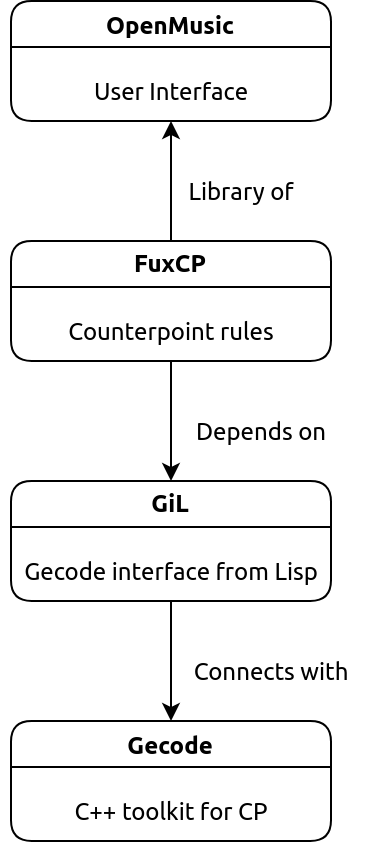
\includegraphics[height=4.4in, center]{Images/macro_arch.png}
  \caption{Macro architecture, overview of the links between FuxCP and the other tools.}
  \label{fig:macro_arch}
\end{figure}
\begin{figure}[h]
  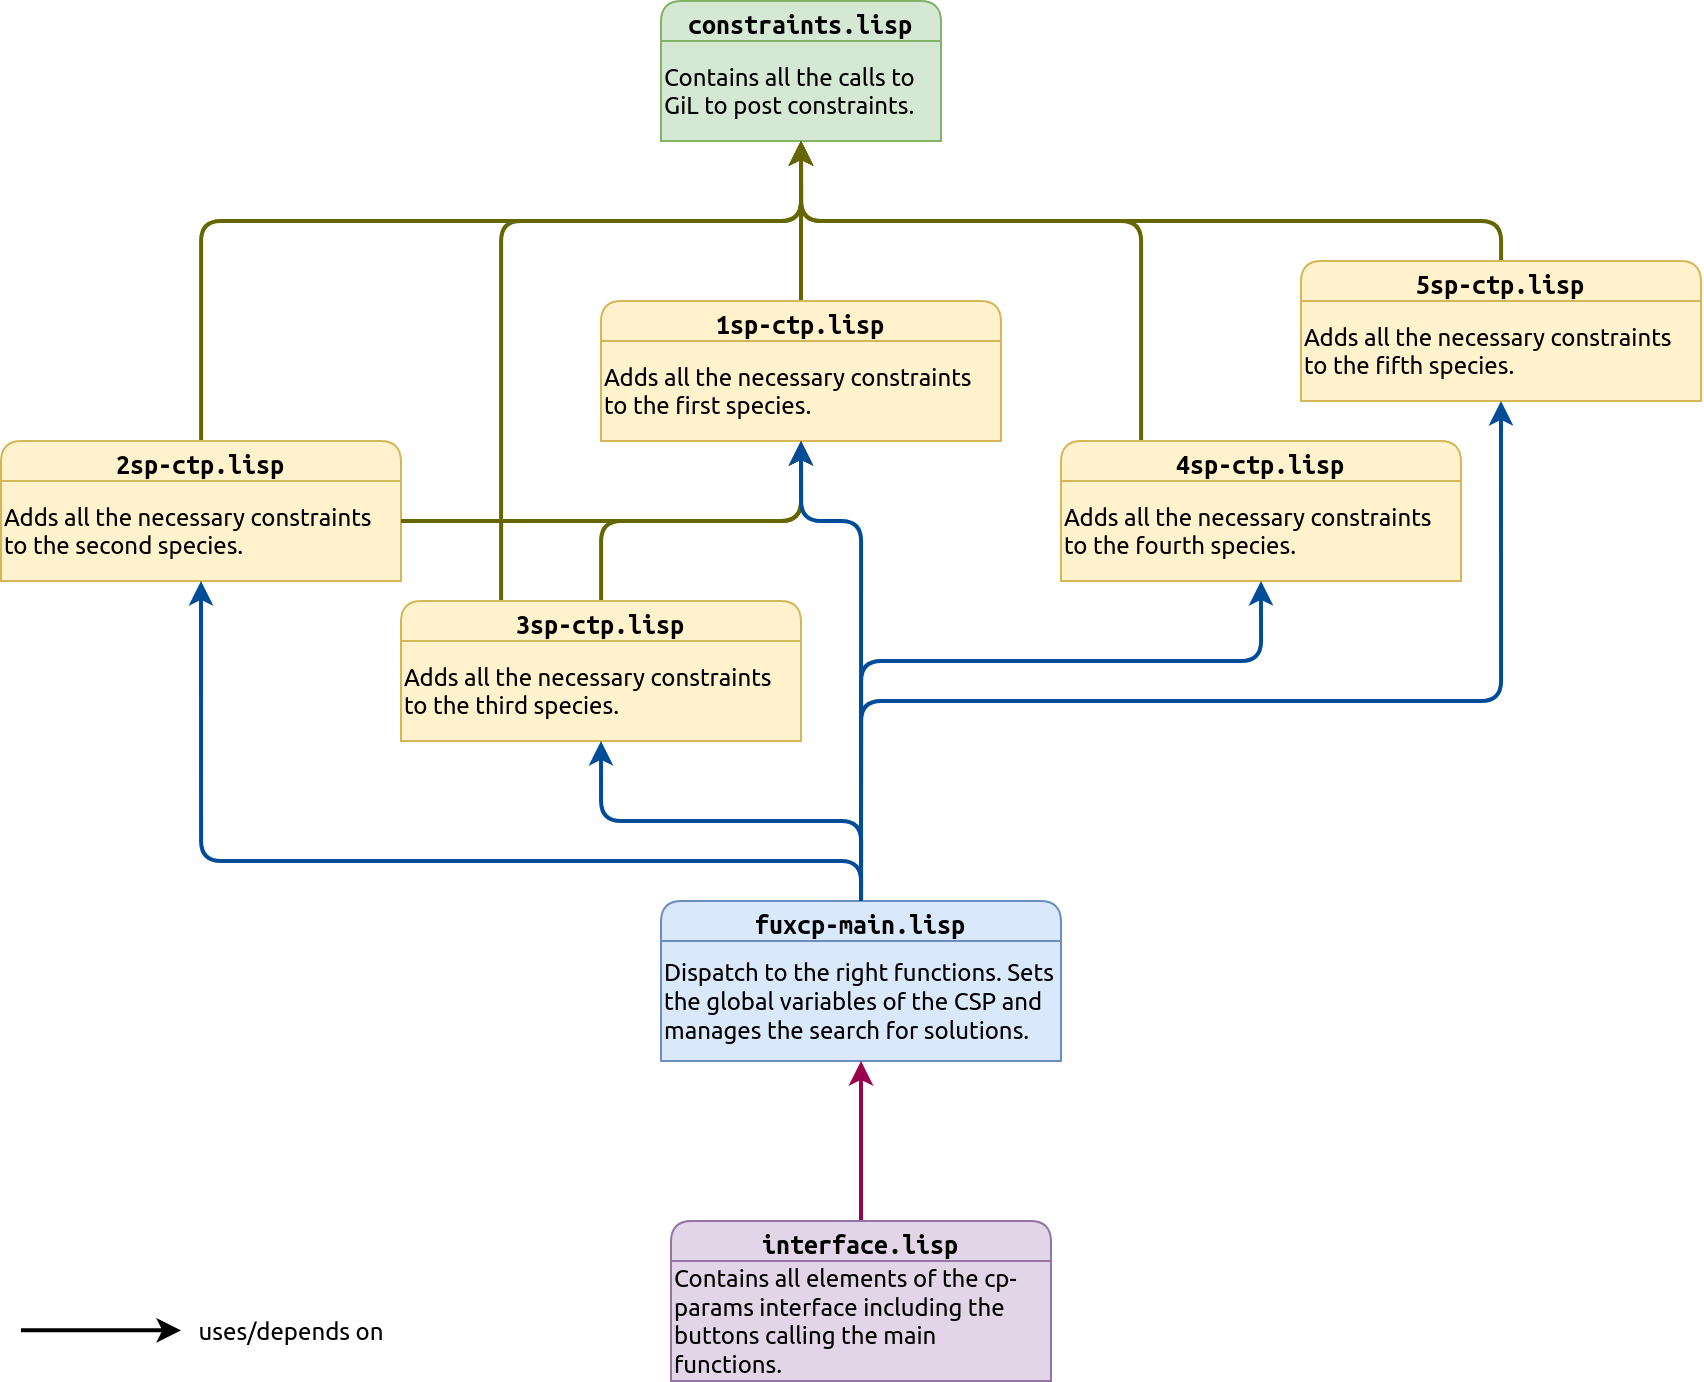
\includegraphics[width=1.2\textwidth, center]{Images/micro_arch.png}
  \caption{Micro architecture, overview of the links between the files.}
  \label{fig:micro_arch}
\end{figure}

\newgeometry{left=1in,right=0.8in,top=0.7in,bottom=0.7in}

\chapter{Source Code}
\section{FuxCP.lisp}
\lstinputlisting{../FuxCP/FuxCP.lisp}
\section{package.lisp}
\lstinputlisting{../FuxCP/sources/package.lisp}
\section{interface.lisp}
\lstinputlisting{../FuxCP/sources/interface.lisp}
\section{fuxcp-main.lisp}
\lstinputlisting{../FuxCP/sources/fuxcp-main.lisp}
\section{1sp-ctp.lisp}
\lstinputlisting{../FuxCP/sources/1sp-ctp.lisp}
\section{2sp-ctp.lisp}
\lstinputlisting{../FuxCP/sources/2sp-ctp.lisp}
\section{3sp-ctp.lisp}
\lstinputlisting{../FuxCP/sources/3sp-ctp.lisp}
\section{4sp-ctp.lisp}
\lstinputlisting{../FuxCP/sources/4sp-ctp.lisp}
\section{5sp-ctp.lisp}
\lstinputlisting{../FuxCP/sources/5sp-ctp.lisp}
\section{constraints.lisp}
\lstinputlisting{../FuxCP/sources/constraints.lisp}